\documentclass[a4paper,10pt]{report}
\usepackage[utf8]{inputenc}
\usepackage[pdftex]{graphicx}
\usepackage{wrapfig}

%opening
\title{CM30225 Parallel Computing\\Assessed Coursework Assignment 2\\Report}
\author{Dominic Hauton}

\begin{document}

\maketitle

\begin{abstract}
A scalability investigation on the proposed parallel matrix relaxation algorithm. Explores Amdahl and Gustaffson and how various metrics change as the size of the problem changes.
\end{abstract}

\section{Code}

The source code is included is structured in three folders:
\begin{itemize}
 \item \emph{matrix} - Responsible for all matrix creation, access and destruction.
 \item \emph{benchmarking} - Contains functions that are used to time and benchmark smooth operations.
 \item \emph{smoothing} - Contains the main loop for for smoothing the matrix.
\end{itemize}
All code is structured using opaque pointers to encapsulate structures and lower coupling, resulting in increased readability and maintainability. Tightly coupled code is often more faster, however, gcc should be able to optimise a lot of function calls.

Compilation is done using cmake. The target system must support AVX instructions as Intel Intrinsic Instructions are used for SWAR acceleration.

\section{MPI - Parallelism}

MPI allows for distributed memory parallelism by sending messages between processes. These processes can be run on one or more MPMD (Multiple Program Multiple Data) machine. The scheduler allows these processes to communicate between each other. As each process has it's own local data, there are no issues with concurrent memory access and cache invalidation present in shared memory systems.\par
The presented solution has 3 main stages:
\begin{itemize}
 \item Scatter
 \item Share
 \item Gather
\end{itemize}\par
\subsection{Scatter}
When a matrix is created using \emph{mat\_factory.c} on the master node. It can then be scattered evenly to every process. \emph{MPI\_Scatterv()} is used to allow MPI to decide how best to distribute the information. The original matrix is split into blocks that need to be computed, and an extra row is added above and below. This is then scattered.
\subsection{Share}
After every iteration the data needs to be shared between the processes. Using non-blocking communication allows MPI to schedule incoming and outgoing information itself and means that, depending on the MPI implementation used, these transfers can be performed in parallel, saving time.

The compute edge rows (top and bottom rows of the computed block) need to be sent to the process computing the section above and below and placed in their outer edge rows (top and bottom rows of the full matrix). The first and last compute section do not send or update their top and bottom rows respectively.

The compute sections need to agree on whether another iteration is required, by ANDing their another computation required flags. If any one section needs to re-smooth, they all need to re-smooth. This is implemented using a \emph{MPI\_Iallreduce()}. This allows MPI to optimise communication between nodes itself and can be done in parallel with the other communication if possible. It also has the benefit of being able to synchronise all of the processes at the end of a loop.
\subsection{Gather}
When all the processes stop needing more iterations all the matrix sections are gathered together and the local matrices are destroyed. Only the computed rows are reassembled at the master node to reduce data throughput required. The MPI command \emph{MPI\_Gatherv()} is used to allow MPI to optimise this operation.
\subsection{Overhead Mitigation}
Three methods of minimise overhead were used:
\subsubsection{Data Reduction}
The data transferred every iteration was minimised to the two required rows and only to the relevant hosts. This resulted in a maximum of 5 transfers per iteration. During the initial scatter all of the data required is sent out in one transaction and in the gather the minimum data required is gathered back in one transaction.
\subsubsection{Native MPI}
The use of native MPI commands such as \emph{MPI\_Scatterv()} utilises the expertise of MPI developers to maximise the performance of the scatter and simplifies the application code. It allows MPI to perform optimisations, such as sending larger data chunks to nodes that are closer, or in the case of \emph{MPI\_Iallreduce()}, allows the reduction and broadcast to happen in a divide and conquer approach.
\subsubsection{Nonblocking MPI}
Using non-blocking MPI commands for the sharing step allows MPI to schedule to communication itself and decide when best to perform tasks such as copying data from the buffer to the pointer for example. This allows communication to be asynchronous and parallel where possible.

\section{Correctness Testing}
\subsection{Sequential vs. Parallel Comparison}
I could assert that my sequential algorithm worked on small sized matrices by printing out the matrix using the mat print function in mat.c for the final and tmp matrix. Using a comparison by eye I could observe that all the values in the matrix, which were previously 0.0f, had not changed by more than the given amount.

Through using encapsulation and a iterator, I was guaranteed that the iterator would always be correct. I could now infer that my larger matrices when computed sequentially were also correct. I could now compare the results of my parallel calculations to the results of my sequential calculations.

To prevent having to recalculate the sequential matrix every time (which would be very slow), I created a mat crc64 check that used type punning to interpret the doubles in the matrix as long values and add them. This is much faster than adding doubles. Using a combination of the crc64, parity and the number of times the matrix had been smoothed in the run, I was able to assert the different methods had produced the same values. These could also be calculated in parallel using a reduction. Functions for doing this are available in mat.c although they are not used in the submitted program.

An sample of the program output is available in the appendix. The CRC and parity should always match that of the sequential version. A print out of a fully smoothed matrix that began as a matrix with zeros on the inside is also available in the appendix along with the calculated CRC.
\subsection{Matrix Symmetry}
An additional sanity check used to check the correctness of larger matricies was the observation that a matrix that starts with the same number on all the edges, and needs to be smoothed repeatedly will retain the symmetry of the original matrix. This is just a sanity check used for tests when the algorithm is changed in addition to the sequential comparison.

Symmetry was checked by calculating matrix parity in mat.c called \emph{mat parity}, which uses type punning to interpret the doubles from the result as long long values, and repeatedly XORs values against each other. If the matrix is indeed symmetric, every single value will be cancelled out by the equal and opposite value on the other side of the matrix. This could also be calculated in parallel.
\subsection{debug\_print()}
This was activated when a deadlock was encountered. The print that occurred before the program stopping indicated the last known executed line.
\subsection{Timing}
In order to time the program execution, I opted to settle for using wall clock time. Unlike testing this from bash, this allowed me to test smoothing speed in the program without the start-up time for configuring and allocating the matrix. CPU cycles could have been measured, however this value would have been difficult to interpret in a parallel process. The wall clock value may have some error due to leap seconds and load on the system from other processes, however, it proved consistent during testing and gave expected results.

\section{Scalability Investigation}
To conduct my scalability investigation I checked the effect of increasing the problem size and the number of nodes.
\subsection{Methodology}
In order to determine the scalability of the proposed algorithm the time required to smooth the matrix was measured over 5 runs. This time ignores matrix generation time but includes the important initial scatter cost. The matrix generation cost is fixed and irrelevant to the smoothing process and therefore the investigation. This allows the generation to be swapped for a load from file, or even a buffer within the program with no impact on results.

Matrix generation was done from a fixed seed value. To make tests fair the number of smoothing loops required was calculated, and the number of smoothing operations could be calculated by multiplying the inner area of the matrix by smoothing loops.

Each smoothing run printed a line of output which was placed into a spreadsheet and was automatically averaged and using a pivot table various relationships could be plotted. The speedup, efficiency, isoefficiency, overhead, Karp-Flatt metric and processing speed of the solution was calculated within the spreadsheet based on the sequential for each size.

Speed calculation: $$Speed = \frac{Loops * (Matrix\ Size - 2)^2}{Time}$$

Speedup calculation: $$Speedup = \frac{Sequential\ Time}{Parallel\ Time}$$

Efficiency calculation: $$Efficiency = \frac{Speedup}{Processes}$$

Karp-Flatt metric calculation: $$E = \frac{\frac{1}{Speedup} - \frac{1}{Processes}}{1 - \frac{1}{Processes}}$$

Overhead calculation: $$Overhead = Sequential\ Time - (Parallel\ Time + Processes)$$

Isoefficiency calculation: $$Isoefficiency = \frac{1}{1 + \frac{Overhead}{Processes}}$$

These values were then plotted on graphs to explore the relationship of the metrics as conditions changed.
\subsection{Scalability with more Nodes}
The first investigation explores the impact of increasing the number of nodes used to solve the problem.

The speedup of the algorithm should increase with more nodes. There may be a slight decrease in efficiency as more nodes are added, but as all communication is asynchronous there should be a one off cost when the number of nodes goes above one.

To test this the starting matrix was kept constant and the number of processes and nodes was varied. This resulted in four lines showing the speed increase with varying amounts of nodes.

\begin{wrapfigure}{R}{0.6\textwidth}
 \centering
 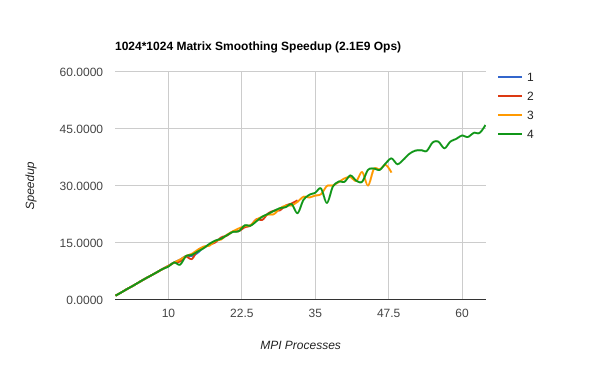
\includegraphics[width=0.6\textwidth]{./images/nodes-speedup.png}
 \caption{Speedup across 1-4 nodes}
 \label{fig:nodespeedup}
\end{wrapfigure}

In figure \ref{fig:nodespeedup} we can see the speedup increasing constantly with a very slight fluctuation when the mpirun was required to run the process on more cores than there were available on one node. However, the impact of this change is very small, much smaller than the noise seen as more processes are used across 3-4 nodes. This is indicative of a very small and constant communication overhead, which does not change if more than one node is used. This may be a sign that MPI is using message passing to communicate between processing instead of memcpy even when on the same node.

\begin{wrapfigure}{L}{0.6\textwidth}
 \centering
 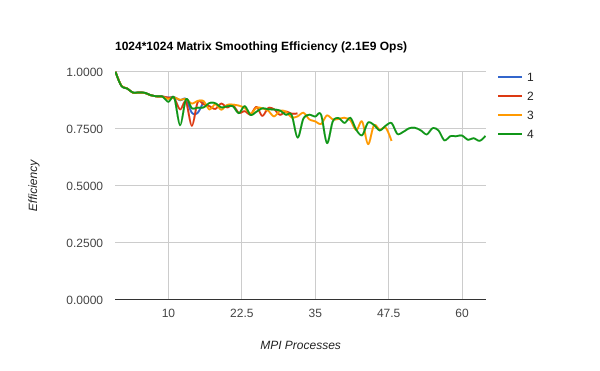
\includegraphics[width=0.6\textwidth]{./images/nodes-efficiency.png}
 \caption{Efficiency across 1-4 nodes}
 \label{fig:nodeefficiency}
\end{wrapfigure}

In the efficiency graph in figure \ref{fig:nodeefficiency} we can see that fairly constant efficiency drop-off as more processes were used, but again no sudden drop off as more nodes were added. This is consistent with the idea that while the communication time is kept constant, there is less and less to do in parallel, so efficiency in the constant time communication lowers the efficiency.

A key observation is that efficiency remains consistent for the same number of MPI processes, regardless of nodes used. This is indicative of mpirun correctly scheduling processes on as few nodes as possible.

As a result of this investigation we can see that the number of nodes does not substantially effect the speed of the algorithm when the number of MPI processes are kept the same. Following this we shall now use 4 nodes during experiments.

\subsection{Scalability with larger matrix}
I second investigation tackles scaling the problem and will also explore different metrics of measuring scalability.

\begin{wrapfigure}{R}{0.45\textwidth}
 \centering
 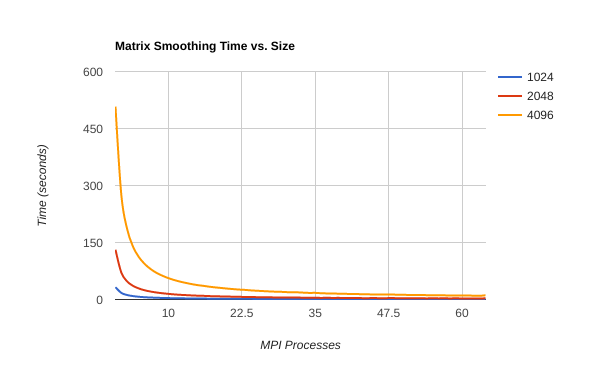
\includegraphics[width=0.45\textwidth]{./images/sizes-time.png}
 \caption{Time across 3 matrix sizes}
 \label{fig:sizestime}
\end{wrapfigure}

According to Gustafson, the speedup of the algorithm should increase as the size of the problem increases. To investigate three sizes of matrix were chosen, each in serial taking four times the length of time that the one before took. A seed for the matrix was chosen that resulted in roughly the same time, and when comparing between matrices of different sizes, we can use the speed metric.

\begin{figure}[!b]
 \centering
 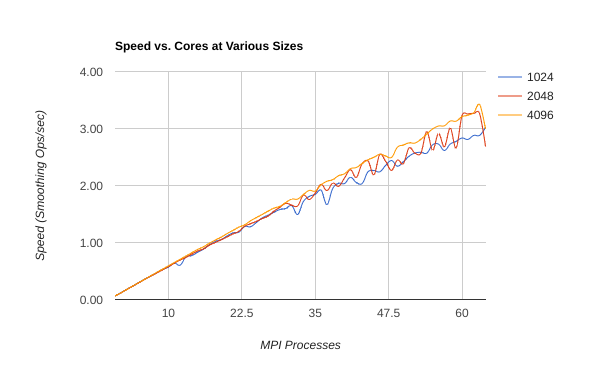
\includegraphics[width=\textwidth]{./images/sizes-speed.png}
 \caption{Speed across 3 matrix sizes}
 \label{fig:sizespeed}
\end{figure}

In figure \ref{fig:sizestime} we can see the computation time decreasing, following the curve of a rational function. This is expected in a parallel algorithm. To be able to observe how fast the nodes are actually processing data, we need to look at the raw processing speed. We use the speed equation to find how many smoothing operations had to be done for the smooth to complete.

Figure \ref{fig:sizespeed} gives us our first glimpse of two important trends in the data. Larger data sets tend run at a faster speed, more calculations are done per second while the algorithm is running, and this discrepancy grows as more MPI processes are used. This is most likely due to the fact that individual cores need to stop less often for reductions and can run at a faster speed because of it.

\begin{figure}[!t]
 \centering
 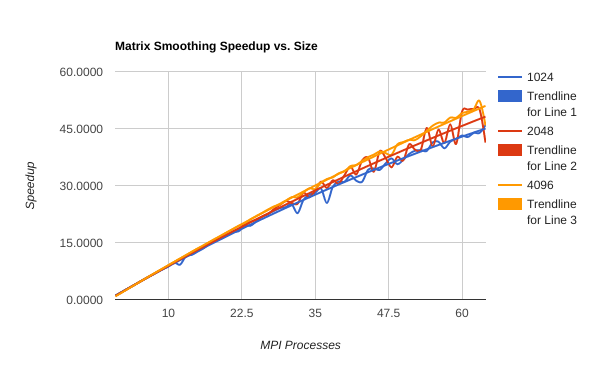
\includegraphics[width=\textwidth]{./images/sizes-speedup.png}
 \caption{Speedup across 3 matrix sizes}
 \label{fig:sizespeedup}
\end{figure}

To explore this relationship further the speedup was also plotted in figure \ref{fig:sizespeedup}. This follows the same trend as the raw speed, but now showing it in terms of the original sequential speed. This allows us to see how much each extra process is helping. An ideal speedup would speed up by one for every extra process added. Here we see that the speedup is closer to ideal with larger matrix sizes, and importantly the more processes we add the less each next one helps.

\begin{wrapfigure}{R}{0.5\textwidth}
 \centering
 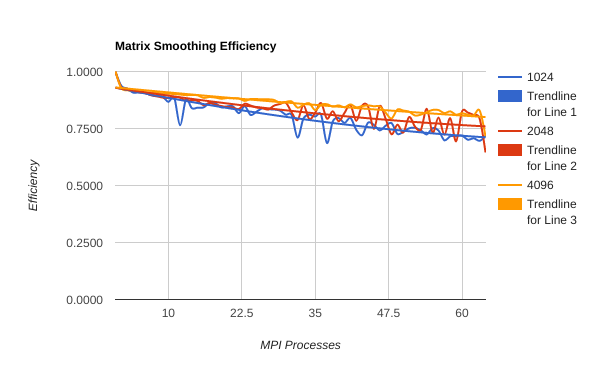
\includegraphics[width=0.5\textwidth]{./images/sizes-efficiency.png}
 \caption{Efficiency across 3 matrix sizes}
 \label{fig:sizesefficiency}
\end{wrapfigure}

Efficiency shows how much each process running in a distributed algorithm helps on average, in comparison to solving the problem sequentially. Efficiency is calculated per problem size and as a result gives us information on scaling for that specific problem size. In figure \ref{fig:sizesefficiency} we see efficiency dropping off with more processes. This can be attributed for the parallel computation time decreasing as the amount of the problem given to each node decreases. Trend lines are added to show the pattern more clearly as the data is noisy.

The efficiency drops at a slower rate for a larger starting problem. This follows on from the previous argument, as the longer a process can work without communication, the more efficient the algorithm is.

Using efficiency information we can proceed to work out the Karp-Flatt metric for the problem. It gives us an indication of how much of the solution is inherently sequential. The higher the number, the larger the part of the problem that is sequential.

\begin{figure}[!t]
 \centering
 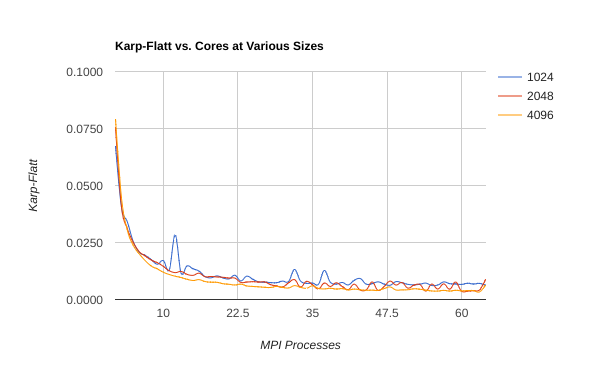
\includegraphics[width=\textwidth]{./images/sizes-karpflatt.png}
 \caption{Karp-Flatt across 3 matrix sizes}
 \label{fig:sizeskarpflatt}
\end{figure}

In figure \ref{fig:sizeskarpflatt} we observe that the more processes, the smaller the inherent sequential time of the process. It is easier than working out what the parallel part of the calculation is in Amdahls law. Usually, the trend with Karp-Flatt is the the sequential overhead is either fixed, or increasing. A decreasing overhead is indicative of decreasing sequential overhead in the program. I suspect this is an artefact of an optimisation put in place that stops calculating diffs between the old and new matrix when the first diff that passes the limit is found.

The faster algorithm removes quite a few operations per smooth speeding up the smoothing process. The sooner all the algorithms can go into the faster algorithm the faster the calculation on every process.

\begin{wrapfigure}{R}{0.5\textwidth}
 \centering
 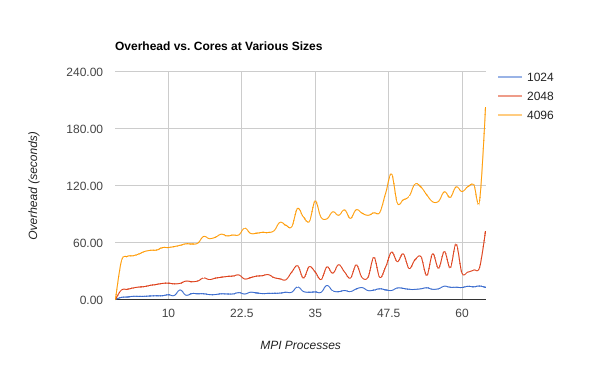
\includegraphics[width=0.5\textwidth]{./images/sizes-overhead.png}
 \caption{Overhead across 3 matrix sizes}
 \label{fig:sizesoverhead}
\end{wrapfigure}

Another possible explanation is that the initial scatter and final gathering of the data can happen in parallel. This scatter can be done in parallel to all processes at once from the master, and the data transfer is smaller for each process lowering the data transmission time. (Send 10MB ten times simultaneously, instead of 100MB once.) As long as the interface/s from the master node are not saturated, this would result in a speedup.

We can deduce that communication is not the bottleneck in the parallelism of our program.

Overhead is a comparison of total compute time on a parallel algorithm. The overhead in figure \ref{fig:sizesoverhead} is exactly what would be expected in this algorithm. The larger the problem, the longer the time required to transfer data between nodes every cycle. In addition the more nodes there are the more overhead there is, as reductions require all nodes to wait for each other. Reductions take longer for a larger amount of nodes.

Finally we have a look at the isoefficiency of the problem. Isoefficiency allows us to find out how much we have to increase to problem size to retain efficiency. This function determines the ease with which a parallel system can maintain a constant efficiency and maintain speedup.

\begin{figure}[!t]
 \centering
 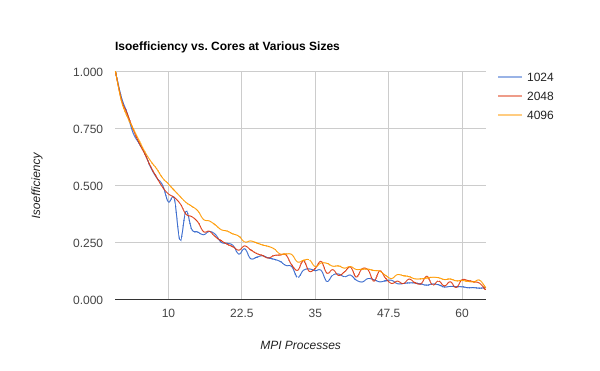
\includegraphics[width=\textwidth]{./images/sizes-isoefficiency.png}
 \caption{Isoefficiency across 3 matrix sizes}
 \label{fig:sizesisoefficiency}
\end{figure}

A small isoefficiency means that small increments in problem size are sufficient to maintain scalability. In figure \ref{fig:sizesisoefficiency} we can observe that the higher the thread count, the less the size needs to be increased to scale. This is consistent with the diverging efficiency between different problem sizes we see at the start. The more work given in each superstep to each node the more efficient it can be.

\section{Other Parallelism}
\subsection{SWAR}
Using SIMD Intel Intrinsics functions from the AVX instruction set I was able to achieve a 350\% speedup in the program, however, as this also speeds up the sequential version the speedup with SWAR was taken into account during analysis. A brief run shows slightly worse speedup with lower matrix sizes in a distributed algorithm with efficiency dropping down to 0.5 at 64 cores with a size of 4096. This is due to the superstep parallel proportion of the calculation taking up much less time proportionally. This is reflected in the now stable Karp-Flatt metric of 0.025 - 0.015 (Although this still decreases as cores increase).

\section{Conclusion}
The solution presented scales well across multiple nodes using a super step pattern of computation.

Further work could be done to reduce communication overhead. One such modification would be transferring more than the rows required, to allow the node to do two extra row calculations instead of asking a neighbouring node for data. This wasn't done as the Karp-Flatt calculation indicated that communication was not an issue.

The analysis shows that the solution efficiency drops as expected, with larger data sets resulting in faster speedup as predicted by Gustafson, and efficiency dropping as more nodes were used, as predicted by Amdahl.

Using Amdahl's Law and the value that the Karp-Flatt metric tended towards we can calculate the maximum processors we can use for speedup. This would be around 0.004 sequential for 2048 and 4096 and as a result $$Max\ speedup(2048/4096) = \frac{1}{Sequential\ Ratio} = \frac{1}{0.004} = 250$$

\section{Appendix}

Included as a separate pdf. An excerpt of the raw results has been provided as a CSV.

\end{document}
